\section{The capacity obstruction}\label{sec:obstruction}
The positive construction reserves more service for an old job when a smaller maximum-flow factor is requested. We now show that the associated capacity conflict is not peculiar to that construction. Below $1/(1-\rho)$, any eligible policy must finish a large busy-cycle root fast enough to leave an order-proportional number of bounded jobs waiting.

The proof separates three statements that can otherwise be confused. A law of large numbers gives a likely finite arrival event. A pathwise competitive guarantee applies to the finite input on that event. A regenerative reward identity converts the resulting delayed-job count into a stationary tail probability. The stochastic event is not an adversarial policy action, and a finite-prefix guarantee is not assumed for a policy with future-horizon information.

\subsection{Uniform laws of large numbers on a growing interval}
After the root arrives, let $N(t)$ count subsequent arrivals, let $A(t)$ be their aggregate work, and, for a fixed $K<\infty$, define
\begin{equation}\label{eq:bounded-work}
 A_K(t)=\sum_{0<a_i\leq t}B_i\ind\{B_i\leq K\},
 \qquad
 \rho_K=\lambda\E[B\ind\{B\leq K\}].
\end{equation}
This is the work of jobs whose \emph{entire} size is at most $K$. It is not the workload obtained by replacing every size with $B\wedge K$. The distinction will be needed when converting unfinished work into a count of unfinished bounded jobs.

\begin{lemma}[A growing-interval event]\label{lem:uniform-lln}
Fix $K<\infty$, $\kappa<\infty$, and $e>0$. For every $b>0$, let $E_b$ be the event that simultaneously for $0\leq t\leq\kappa b$,
\begin{align}
 |A(t)-\rho t|&\leq eb,\label{eq:event-A}\\
 |A_K(t)-\rho_Kt|&\leq eb,\label{eq:event-AK}\\
 |N(t)-\lambda t|&\leq eb.\label{eq:event-N}
\end{align}
Then $\Pp(E_b)\to1$ as $b\to\infty$. The statement also holds for the left limits of these paths.
\end{lemma}
\begin{proof}
The Poisson strong law gives $N(t)/t\to\lambda$ almost surely. Applying the iid strong law to the marks along the arrival sequence gives $A(t)/t\to\lambda\mu=\rho$. The same argument applied to $B\ind\{B\leq K\}$ gives $A_K(t)/t\to\rho_K$. Only finite means are needed.

For any one of these paths $Z$ with rate $z$, write $R(t)=Z(t)-zt$. If $R(t)/t\to0$, then $b^{-1}\sup_{0\leq t\leq\kappa b}|R(t)|\to0$. To see this, choose a deterministic tolerance $\xi>0$ and, on the almost-sure convergence event, a finite random time $t_0$ after which $|R(t)|\leq\xi t$. Before $t_0$, the path is bounded because there are finitely many arrivals on compact intervals. Therefore
\[
 \frac1b\sup_{t\leq\kappa b}|R(t)|
 \leq\frac1b\sup_{t\leq t_0}|R(t)|+\xi\kappa.
\]
Take $b\to\infty$ and then $\xi\downarrow0$. Apply this to all three paths. Bounds for left limits follow by approaching a jump time from below. Almost-sure convergence of the scaled suprema implies the asserted probability convergence.
\end{proof}

The future marked Poisson process is independent of the root's size. Consequently, the event probabilities in this lemma are the same when we condition on that size being $b$. Moreover, convergence as a real parameter $b\to\infty$ implies that the infimum of these probabilities over $b\geq b_0$ tends to one as $b_0\to\infty$. No discretization of the root size is needed.

\subsection{An order-proportional delayed cohort}
\begin{lemma}[Finite-prefix capacity deficit]\label{lem:deficit}
Fix $C\geq1$ with $C<1/(1-\rho)$. There are constants $K<\infty$, $\kappa>C$, $e>0$, $\eta>0$, and $c_0>0$, depending only on the environment and $C$, such that the following holds.

Start an eligible $C$-competitive policy from an empty queue with a root of size $b>K$ at time zero. On the event $E_b$ of Lemma~\ref{lem:uniform-lln}, at least $c_0b$ jobs from that same busy cycle have response greater than $\eta b$.
\end{lemma}
\begin{proof}
Since $\rho_K\uparrow\rho$ and $C<1/(1-\rho)$, choose $K\geq1$ such that
\begin{equation}\label{eq:K-choice}
 \rho_K>1-1/C.
\end{equation}
Choose $\kappa$ strictly between $C$ and $1/(1-\rho_K)$, and set
\begin{equation}\label{eq:Delta}
 \Delta=1-\kappa(1-\rho_K)>0.
\end{equation}
Use the explicit positive constants
\begin{align}
 e&=\min\left\{\frac{\kappa/C-1}{4},\frac\Delta4,
                  \frac\Delta{16K},\frac18\right\},\label{eq:epsilon-choice}\\
 \eta&=\min\left\{\frac\kappa2,
                   \frac\Delta{8K(\lambda+1)}\right\},
 \qquad c_0=\frac\Delta{2K}.\label{eq:eta-choice}
\end{align}
In particular,
\begin{equation}\label{eq:constant-inequalities}
 C(1+2e)<\kappa,
 \qquad e\leq\Delta/4,
 \qquad\lambda\eta+2e\leq\Delta/(4K).
\end{equation}
The first inequality follows from $C(1+2e)\leq(C+\kappa)/2<\kappa$. The last follows by bounding its two terms separately by $\Delta/(8K)$.

Put $H=\kappa b$. Consider the finite input consisting of the root and all arrivals through $H$. On $E_b$, its unit-speed workload is at most $(1+2e)b$ by~\eqref{eq:fluid-opt}. Its workload decreases after $H$, so Lemma~\ref{lem:workload} gives
\begin{equation}\label{eq:prefix-opt}
 \OPT(I^{H})\leq(1+2e)b.
\end{equation}
The competitive guarantee on this \emph{finite} input forces the root to complete by $C(1+2e)b<H$. By prefix consistency, its execution through $H$ is the same in the true queue. Hence the root also completes before $H$ there.

The initial busy period does not end before $H$. If it first ended at some $t\leq H$, work conservation up to that time would give zero net work. But on $E_b$,
\begin{align*}
 b+A(t)-t
 &\geq b+A_K(t)-t\\
 &\geq b-(1-\rho_K)t-eb\\
 &\geq(\Delta-e)b>0,
\end{align*}
contradicting such an empty time. Thus every arrival used below belongs to the root's busy cycle.

By time $H$, the root has received $b$ service. Therefore the service given to subsequent bounded jobs is at most $H-b$, regardless of how much service any other large jobs receive. Their remaining work is at least
\begin{align}
 A_K(H)-(H-b)
 &\geq\rho_KH-eb-H+b\notag\\
 &=(\Delta-e)b\geq\frac{3\Delta}{4}b.\label{eq:remaining-bounded}
\end{align}
Each such unfinished job has total size at most $K$, so there are at least $3\Delta b/(4K)$ of them. This implication would be invalid for untruncated jobs; one arbitrarily large residual could otherwise account for all the work.

The number of arrivals after $H-\eta b$ and through $H$ is at most
\begin{equation}\label{eq:recent-count}
 N(H)-N(H-\eta b)
 \leq(\lambda\eta+2e)b\leq\frac\Delta{4K}b.
\end{equation}
Subtract even all of these recent arrivals from the unfinished bounded-job count. At least $\Delta b/(2K)$ unfinished jobs remain; this quantity is $c_0b$ whose releases are at or before $H-\eta b$. Because they are unfinished at $H$, each has eventual response strictly greater than $\eta b$. Their busy cycle is finite almost surely under the stable work-conserving workload, so these are ordinary finite responses counted in that cycle.
\end{proof}

The lemma does not require that the root be served continuously, be the oldest job chosen for priority, or remain unfinished until near $H$. It only requires that the finite-input guarantee make the policy finish the root before $H$. The rest is service accounting. The same accounting remains valid when current sizes are revealed to the policy.

\subsection{Why truncation and regeneration are both necessary}\label{sec:truncation-regeneration}
The truncation at $K$ and the restriction to one root per busy cycle solve different problems.  Truncation is a \emph{volume-to-count} device.  A lower bound on unfinished work alone does not imply that many customers are delayed: one exceptional residual could contain all of that work.  By retaining only jobs whose total size is at most $K$, equation~\eqref{eq:remaining-bounded} converts residual volume into at least residual volume divided by $K$ unfinished jobs.  This is why replacing $B\ind\{B\leq K\}$ by $B\wedge K$ would be incorrect: a very large job would then contribute artificial bounded work although it is still only one customer.

Regeneration is a \emph{double-counting} device.  Heavy-tailed busy periods and workloads are often governed by a one-large-job mechanism~\cite{zwart2001,abate1994,boxmadenisov2011}.  Selecting every large arrival in stationary time, however, would produce overlapping future windows and would not by itself identify how many distinct delayed arrivals should be credited to each trigger.  We instead inspect only the first job of each busy cycle.  Its mark has the ordinary law $F$, its future marked Poisson process is independent, and every delayed job produced by Lemma~\ref{lem:deficit} belongs to that same finite cycle.  The random variables $Q_x$ below therefore partition delayed arrivals by cycles rather than by possibly overlapping large-job events.

The cycle argument is an arrival-average statement, not a time-average queue-length statement.  Palm and regenerative methods distinguish these averages in general~\cite{baccelli2003,wolff1982}.  Here the reward is literally the number of arrivals in a cycle whose eventual responses exceed $x$.  Dividing expected reward by the expected number of arrivals in a cycle gives the typical-arrival probability.  Integrating the number of delayed jobs present over time would instead produce a response-time moment through Little's law and would require different integrability assumptions.  The count reward avoids any need for $\E T<\infty$.

These choices also explain the scale of the lower bound.  A root in a window of probability order $\Fbar(x)$ forces order $x$ delayed arrivals; the product is $x\Fbar(x)$.  Classical integrated-tail formulas motivate this scale, but they do not prove the policy-independent cohort in Lemma~\ref{lem:deficit}.  That cohort comes from the finite-input deadline and the bounded-job capacity deficit.

\subsection{From busy-cycle rewards to stationary tails}
Let $V$ be the number of jobs in a busy cycle, starting with the first arrival to an empty queue, and let $Q_x$ be the number among them whose response exceeds $x$. We need the arrival version of the regenerative reward formula, not a time average of the number of delayed jobs in service.

\begin{lemma}[Cycle count and arrival reward]\label{lem:cycle-reward}
For the stable unit-speed M/G/1 queue and any eligible policy,
\begin{equation}\label{eq:cycle-count}
 \E V=\frac1{1-\rho},\qquad
 \Pp(T>x)=\frac{\E Q_x}{\E V}=(1-\rho)\E Q_x.
\end{equation}
\end{lemma}
\begin{proof}
The work-conserving workload determines busy-period endpoints independently of the service order. Its job count can therefore be computed under FCFS. Regard arrivals during a job's service as that job's children. Conditional on a size $B$, the offspring count is Poisson with mean $\lambda B$. The independent marked Poisson construction gives a branching description with offspring mean $\rho<1$. The expected number in generation $j$ is $\rho^j$. Summing these expectations by monotone convergence gives $\E V=\sum_{j\geq0}\rho^j=1/(1-\rho)$.

Under the policy's empty-state reset and time-shift invariance, consecutive busy cycles, together with intervening idle times, are regenerative. Count arrivals with response greater than $x$ over complete cycles and divide by the total number of arrivals over those cycles. The regenerative strong law gives the ratio $\E Q_x/\E V$. This is the probability for a typical stationary arrival. The required reward is integrable because $0\leq Q_x\leq V$ and $\E V<\infty$. No finite mean of $T$, no second moment of $V$, and no second service moment are used.
\end{proof}

\begin{theorem}[Integrated-tail obstruction]\label{thm:obstruction}
Fix a regularly varying finite-mean M/G/1 environment with $\rho\in(0,1)$. Let an eligible policy have a finite maximum-flow competitive factor $C<1/(1-\rho)$. With the constants in Lemma~\ref{lem:deficit},
\begin{equation}\label{eq:lower-constant}
 \liminf_{x\to\infty}
  \frac{\Pp(T>x)}{x\Fbar(x)}
 \geq (1-\rho)c_0\eta^{\alpha-1}(1-2^{-\alpha})>0.
\end{equation}
The constants can be chosen uniformly over all eligible policies with factor at most this fixed $C$.
\end{theorem}
\begin{proof}
In a busy cycle, the root size has the ordinary law $F$ and is independent of the future marked Poisson process. Restrict its size to
\begin{equation}\label{eq:root-range}
 x/\eta<B\leq2x/\eta.
\end{equation}
For sufficiently large $x$, all these roots exceed $K$. On $E_B$, Lemma~\ref{lem:deficit} gives at least $c_0B\geq c_0x/\eta$ jobs in the same cycle with response greater than $\eta B>x$. The infimum of $\Pp(E_b)$ over $b\geq x/\eta$ tends to one by Lemma~\ref{lem:uniform-lln}. Consequently,
\begin{equation}\label{eq:cycle-lower}
 \E Q_x\geq(1-o(1))\frac{c_0x}{\eta}
       \bigl(\Fbar(x/\eta)-\Fbar(2x/\eta)\bigr).
\end{equation}
Regular variation makes the parenthesized difference asymptotic to
\[
 \eta^\alpha(1-2^{-\alpha})\Fbar(x).
\]
Multiply by $1-\rho$ using Lemma~\ref{lem:cycle-reward} to obtain~\eqref{eq:lower-constant}. Every event and constant in this argument depends only on $C$, $\lambda$, and $F$, not on the policy's prioritization rule.
\end{proof}

The theorem proves a lower bound at the integrated-tail scale because of~\eqref{eq:integrated-tail}. It does not assert an asymptotic equality for every policy. Its immediate implication for the positive objective is stronger than a failure of a particular constant:
\[
 \liminf_{x\to\infty}\frac{\Pp(T>x)}{\Fbar(x)}=\infty.
\]
The linear factor comes from a count of delayed jobs in a cycle. Treating the root's own delay as the entire reward would miss this factor.


When $1<\alpha<2$, the boundary also separates mean response: the
obstruction gives $\E T=\infty$ below $1/(1-\rho)$ because
$x\Fbar(x)\in\RV(1-\alpha)$ is nonintegrable, whereas guarded sharing
above the boundary has $\E T<\infty$ because its tail is
$O(\Fbar(x))$ and $\int_0^\infty\Fbar(x)\,dx=\E B<\infty$.
At $\alpha=2$, this tail-order comparison alone does not decide mean-response integrability.

\subsection{Quantifiers and the remaining boundary}
Together with Theorem~\ref{thm:guard-tail}, Theorem~\ref{thm:obstruction} proves Theorem~\ref{thm:boundary-intro}. Figure~\ref{fig:phase} displays the strict separation. The upper region means that a suitable policy exists, not that every policy with a larger competitive factor has a good tail. A policy can always have a loose advertised factor; the result about exact factors uses Theorem~\ref{thm:guard-tight}.

\begin{figure}[t]
\centering
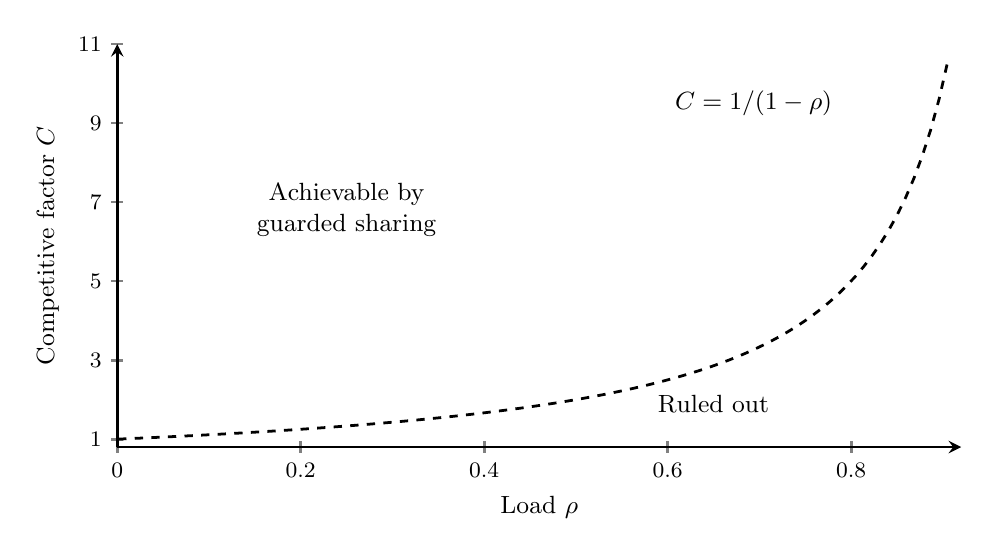
\begin{tikzpicture}
\begin{axis}[
 width=12.3cm,height=6.7cm,
 xmin=0,xmax=.92,ymin=.8,ymax=11,
 xlabel={Load $\rho$},ylabel={Competitive factor $C$},
 xtick={0,.2,.4,.6,.8},ytick={1,3,5,7,9,11},
 axis lines=left,clip=true,
 axis line style={line width=1pt},tick style={line width=1pt},
 tick label style={font=\footnotesize},
 label style={font=\small}]
 \addplot[black,dashed,line width=1pt,domain=.001:.905,samples=100] {1/(1-x)};
 \node[align=center,font=\small] at (axis cs:.25,6.8)
   {Achievable by\\guarded sharing};
 \node[align=center,font=\small] at (axis cs:.65,1.9)
   {Ruled out};
 \node[anchor=east,font=\small] at (axis cs:.79,9.5)
   {$C=1/(1-\rho)$};
\end{axis}
\end{tikzpicture}

\caption{The unit-speed strict boundary. For a fixed load, every competitive factor strictly above the curve is realized by guarded sharing with a job-size-order tail. Factors strictly below it are impossible for eligible policies with that tail guarantee. The curve itself is not classified. The curve is the analytic function $1/(1-\rho)$, not an empirical fit.}\label{fig:phase}
\end{figure}

There are three important exclusions in the converse. A policy that knows the final input horizon need not behave the same on a finite prefix and on an infinite queue, so~\eqref{eq:prefix-opt} cannot be transferred to it without additional work. A message that encodes the future realization likewise invalidates the independence used in~\eqref{eq:cycle-lower}. A bound only in expectation over a policy's randomness does not force pathwise root completion on $E_b$. None is silently included in the theorem.

At $C=1/(1-\rho)$, no finite truncation can satisfy~\eqref{eq:K-choice}: it would require $\rho_K>\rho$. The converse proof therefore stops for a substantive reason. On the positive side, the slower PS comparison would have load one, so its stationary count law cannot be normalized. These two failures do not resolve each other. They identify the equality case as a different question rather than license to replace either strict inequality by a non-strict one.
